\documentclass[14pt, a4paper]{extreport}

\usepackage{susu}

% ====================================================================================================
\begin{document}

\author{Савонин~М.В.}
\group{211}
\task{1}
\maketitle

% ====================================================================================================
\chapter{Задание}

\begin{enumerate}

	\item
	Разработать подпрограммы для градиентной закраски прямоугольной области различными способами.
	Аргументы подпрограмм -- координаты левого верхнего угла, ширина и высота области.
	Подпрограммы должны работать для любого соотношения размеров прямоугольной области.
	Для каждого способа закраски определить зависимость интенсивности цвета от координат точки.
	При реализации подпрограмм использовать для рисования только процедуру putpixel.

	\item
	Написать программу для тестирования разработанных \linebreak подпрограмм.
	Интерфейс программы должен содержать следующие элементы управления:
	\begin{itemize}
		\item выбор способа закраски;
		\item сохранение результата в файл;
		\item выход из программы.
	\end{itemize}

\end{enumerate}

% ====================================================================================================
\chapter{Математическая модель}

Пусть $x_0$, $y_0$, $x_1$, $y_1$ -- соответственно координаты первой точки и второй точки.
При рисовании линии цвет задан изначально color, а координаты простовляемого пикселя x и y.

Рисование линии:
$$ deltax = |x_1-x_0| . $$
$$ deltay = |y_1-y_0| . $$
$$ error = 0 . $$
Если изменение по x больше чем по y:
$$ deltaerr = \frac{deltay}{deltax} . $$
Если $x_0$ больше $x_1$ то меняем значения точек местами.
$$ y = y_0 . $$
\begin{equation*}
diry = \left\{
\begin{array}{lr}
1 & \text{ для } y_1-y_0 > 0 \\
-1 & \text{ для }y_1-y_0 < 0 \\
0 & \text{ для }y_1-y_0 = 0
\end{array}
\right.
\end{equation*}
Проходимся по всем значениям x от $x_0$ до $x_1$ и ставим пиксели заданного цвета:
$$ error = error + deltaerr. $$
При error $\geq$ 1:
$$ y = y + diry . $$
$$ error = error - 1 . $$
Если изменение по y больше или равно изменению по x:
$$ deltaerr = \frac{deltax}{deltay} . $$
Если $y_0$ больше $y_1$ то меняем значения точек местами.
$$ x = x_0 . $$
\begin{equation*}
dirx = \left\{
\begin{array}{lr}
1 & \text{ для } x_1-x_0 > 0 \\
-1 & \text{ для }x_1-x_0 < 0 \\
0 & \text{ для }x_1-x_0 = 0
\end{array}
\right.
\end{equation*}
Проходимся по всем значениям x от $y_0$ до $y_1$ и ставим пиксели заданного цвета:
$$ error = error + deltaerr. $$
При error $\geq$ 1:
$$ x = x + derx . $$
$$ error = error - 1 . $$

% ====================================================================================================
\chapter{Текст программы}

\noindent Файл main.cpp
\lstinputlisting{source/main.cpp}
\pagebreak
\hrulefill

\noindent Файл task.h
\lstinputlisting{source/task.h}
\hrulefill

\noindent Файл task.cpp
\lstinputlisting{source/task.cpp}
\hrulefill

\noindent Файл control.h
\lstinputlisting{source/control.h}
\hrulefill

\noindent Файл control.cpp
\lstinputlisting{source/control.cpp}

% ====================================================================================================
\chapter{Результат работы}

\begin{figure}[h!]
	\centering
	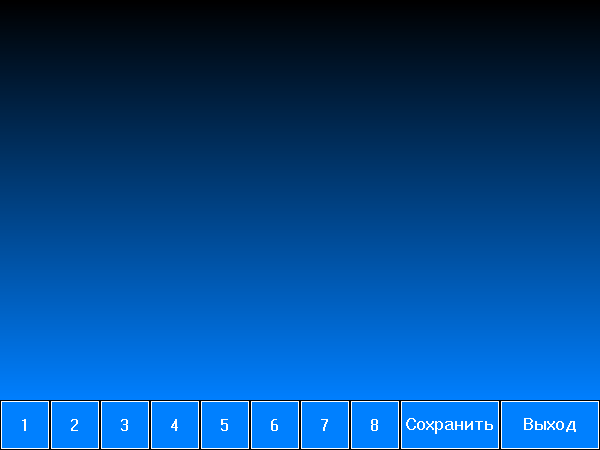
\includegraphics[width = 12cm]{image/image_1}
  \caption{Результат выполнения программы (способ 1)}
\end{figure}

\begin{figure}[h!]
	\centering
	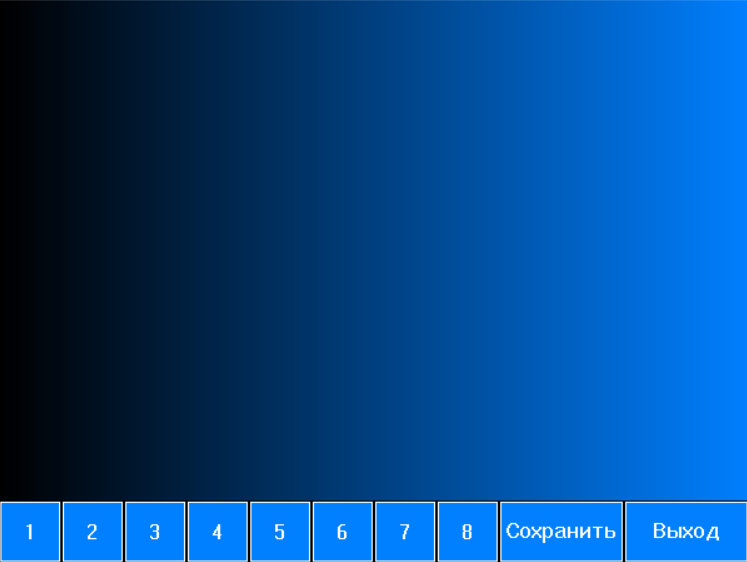
\includegraphics[width = 12cm]{image/image_2}
  \caption{Результат выполнения программы (способ 2)}
\end{figure}

\begin{figure}[h!]
	\centering
	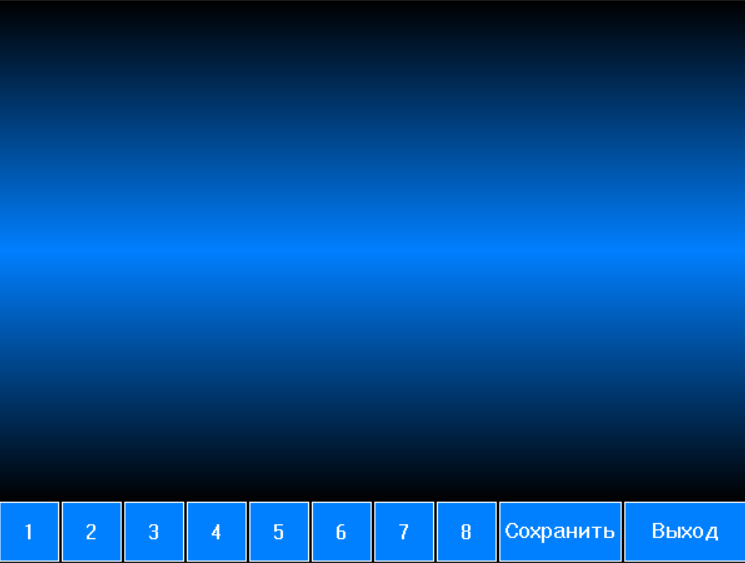
\includegraphics[width = 12cm]{image/image_3}
  \caption{Результат выполнения программы (способ 3)}
\end{figure}

\begin{figure}[h!]
	\centering
	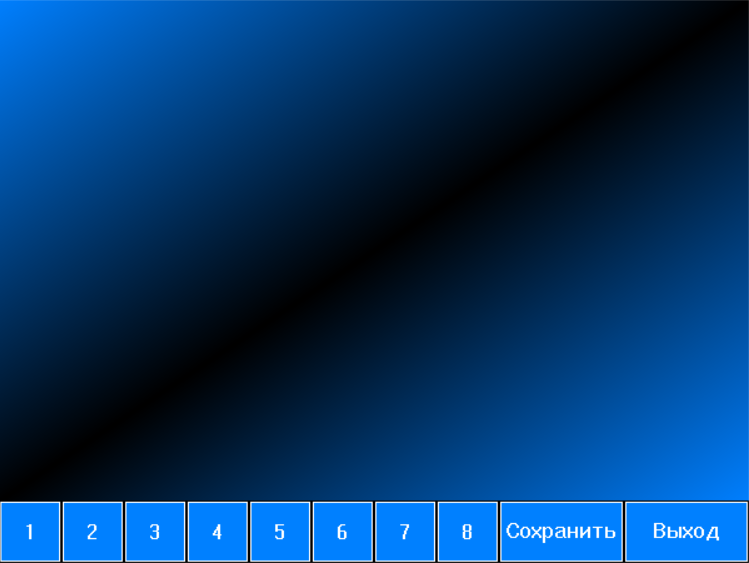
\includegraphics[width = 12cm]{image/image_4}
  \caption{Результат выполнения программы (способ 4)}
\end{figure}

\begin{figure}[h!]
	\centering
	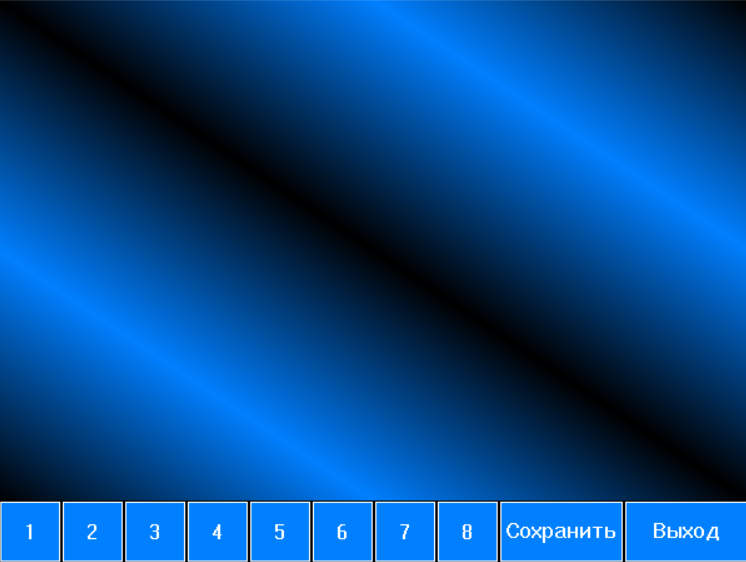
\includegraphics[width = 12cm]{image/image_5}
  \caption{Результат выполнения программы (способ 5)}
\end{figure}

\begin{figure}[h!]
	\centering
	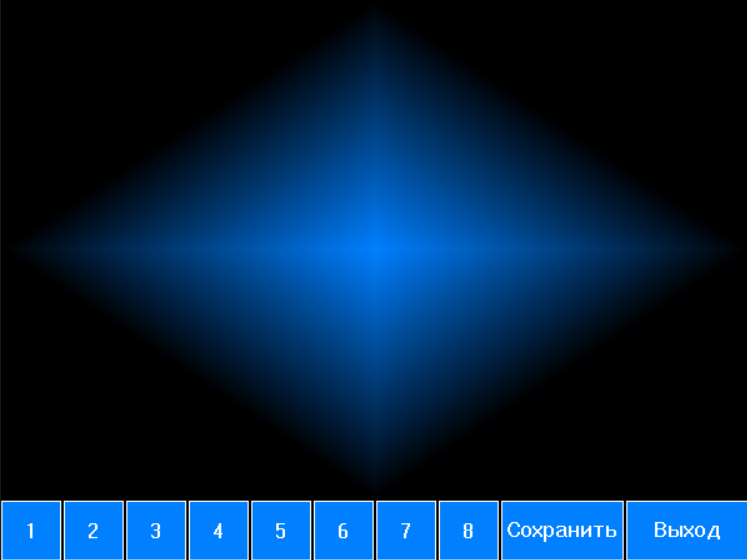
\includegraphics[width = 12cm]{image/image_6}
  \caption{Результат выполнения программы (способ 6)}
\end{figure}

\begin{figure}[h!]
	\centering
	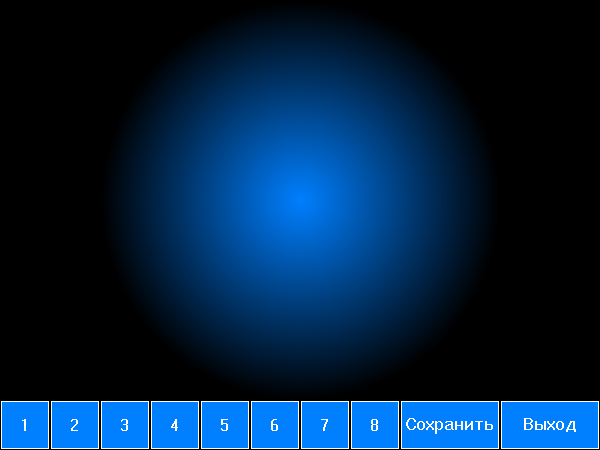
\includegraphics[width = 12cm]{image/image_7}
  \caption{Результат выполнения программы (способ 7)}
\end{figure}

\begin{figure}[h!]
	\centering
	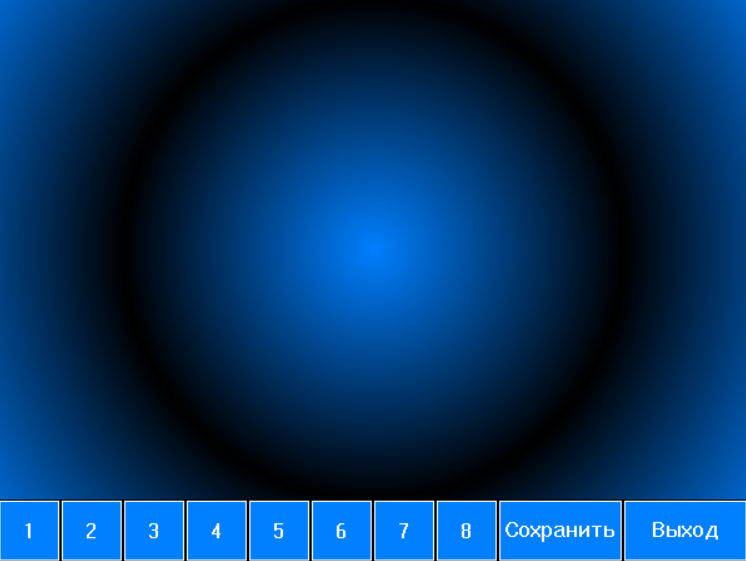
\includegraphics[width = 12cm]{image/image_8}
  \caption{Результат выполнения программы (способ 8)}
\end{figure}

% ====================================================================================================
\end{document}